%% Beispiel-Präsentation mit LaTeX Beamer im KIT-Design
%% entsprechend den Gestaltungsrichtlinien vom Februar 2025
%%
%% Siehe https://sdq.kastel.kit.edu/wiki/Dokumentvorlagen

%% Beispiel-Präsentation
\documentclass[en]{sdqbeamer}
\setbeameroption{show notes on second screen=right}
 
%% Gruppenlogo, muss im Verzeichnis logos/ liegen
%% falls kein Gruppenlogo gewünscht, bitte \grouplogo{} aufrufen
\grouplogo{sdqlogo} 

%% Gruppenname und Breite (Standard: 89 mm)
\groupname{KASTEL - SDQ}
%\groupnamewidth{89mm}

% Beginn der Präsentation

\title[Feature Annotated Reactions Language]{Feature Annotated Reactions Language}
%\subtitle{entsprechend den Gestaltungsrichtlinien von Februar 2025} 
\author[Valentin Kaczmarek]{Valentin Kaczmarek}

\date[9.\,3.\,2026]{9. March 2026}

% Literatur 
 
\usepackage[citestyle=authoryear,bibstyle=numeric,hyperref,backend=biber]{biblatex}
\addbibresource{presentation.bib}
\bibhang1em

\usepackage{lipsum}
\usepackage[final]{listings}
\lstset{basicstyle=\ttfamily}
\usepackage{pgfpages}
\setbeamertemplate{note page}[plain]
\setbeamerfont{note page}{size=\Large}
\setbeamercolor{note page}{bg=white, fg=black}
\usepackage{pgfgantt}

\begin{document}

%Titelseite
\begin{frame}[title green horizontal, picture=images/palladio_bauplan, kitlogo=white]
	\titlepage
\end{frame}

\section{Motivation}

\begin{frame}{Motivation}
	\begin{itemize}
		\item Increasing complexity of software systems \note[item]{distributed knowledge, model driven engineering, consistency gets more important}
		\item Vitruvius for consistency preservation \note[item]{reactions language, trigger on model instance change}
		\item No variability support in reactions \note[item]{methodologist must duplicate rule sets for different configurations, error-prone, scales badly, runtime user prompts can cause inconsistent outcomes}
	\end{itemize}
\end{frame}

\begin{frame}{Reactions}
	\begin{figure}
		\centering
		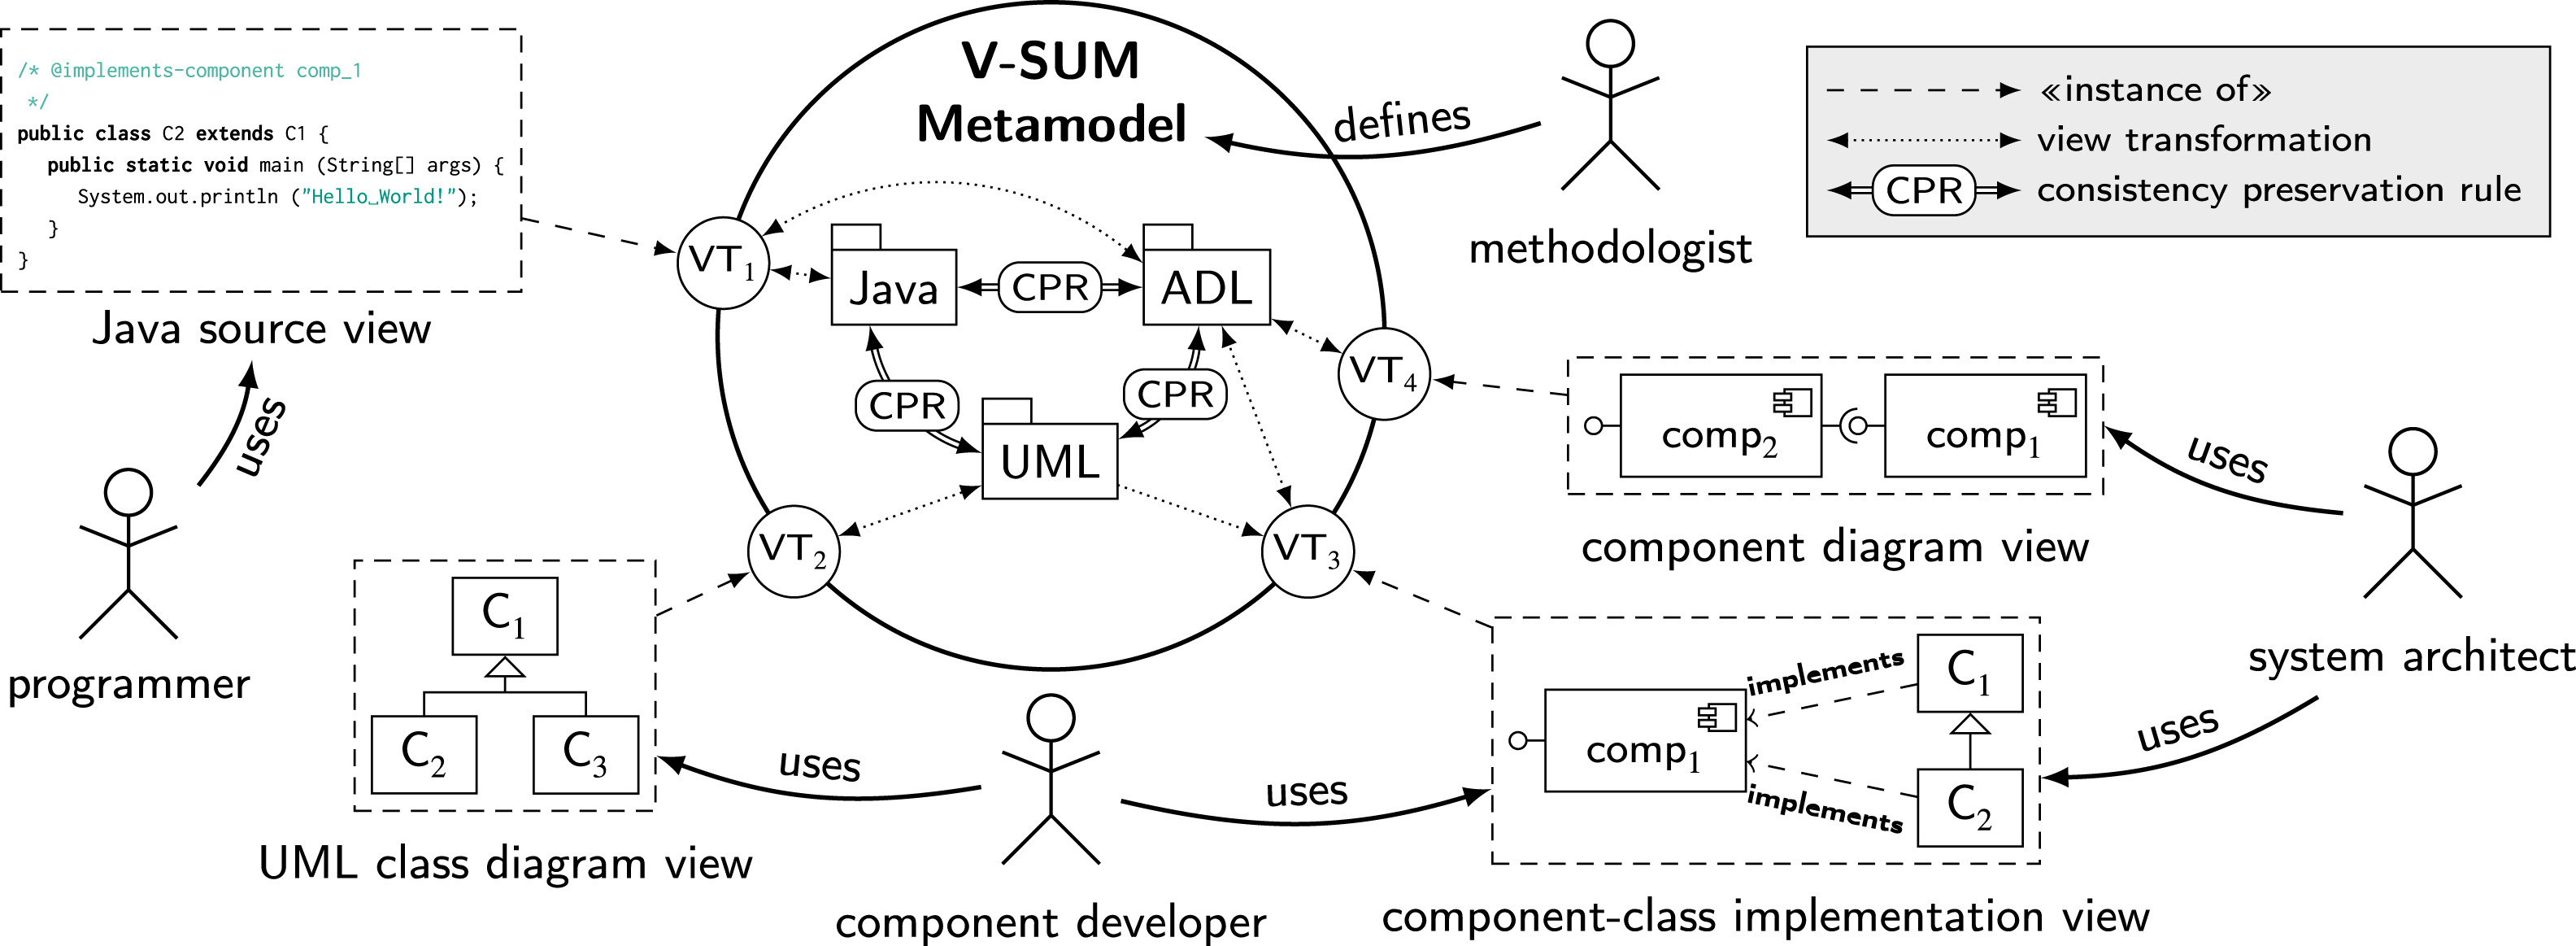
\includegraphics[width=0.9\textwidth]{images/vsum-reactions.jpg}
		\caption{CPR in Vitruvius [\cite{KLARE2021110815}]}
		\label{fig:vitruvius-cpr}
	\end{figure}
	\note[item]{reactions work with bidirectional consistency, trigger on new UML class, reaction uml2java, new Java class}
\end{frame}

\section{PIBA}

\begin{frame}{PIBA}
	\begin{itemize}
		\item Problem: Reaction language restricted \note[item]{one path, hard to adapt, (user interaction) possible inconsistent runs}
		      \pause
		\item Idea: Software product line and feature annotations \note[item]{expand to spl, 150\% model (contains more reactions than needed), enabling variability, annotation selects reaction, provide default for user interaction}
		      \pause
		\item Benefit: More options and less runtime variability \note[item]{precise options to choose, customization easier, no/reduced runtime variability}
		      \pause
		\item Action: Syntax, execution change and more reactions \note[item]{syntax to support annotation (prevent errors in editor), compiler/preprocessor needs to understand annotations, be able to choose reaction, validate with existing and new tests}
	\end{itemize}
\end{frame}

\section{Foundation}

\begin{frame}{Foundation}
	\begin{itemize}
		\item Vitruvius \note[item]{runtime, consistency preservation}
		\item Reactions language \note[item]{logic for updating model instance and keeping consistency}
		\item Eclipse Modelling Framework \note[item]{base for reactions, grammar defined in xtext}
		\item Software Product Line \note[item]{shared set of features, annotations determine specific reaction}
	\end{itemize}
\end{frame}

\section{Related Work}

\begin{frame}{Related Work}
	\begin{itemize}
		\item {}[\cite{KLARE2021110815}] Enabling consistency in view-based system development — The Vitruvius approach \note[item]{do not talk about}
		\item {}[\cite{struber2018variability}] Variability-based model transformation: formal foundation and application \note[item]{base for variability points, similar rules into a compact representation}
		\item {}[\cite{santos2015ifdef}] Do \#ifdef-based variation points realize feature model constraints? \note[item]{ifdef preprocessor statement for conditional compilation, only relevant code as a result}
		\item {}[\cite{barkowsky2023incremental}] Incremental model transformations with triple graph grammars for multi-version models \note[item]{works on multiple versions of a model at the same time, promises higher speed}
	\end{itemize}
\end{frame}

\section{Concept}

\begin{frame}[fragile]{Concept}
	\lstinputlisting[frame=single, caption={Existing reaction {[\cite{umljavacasestudy}]}}, label=listing:existing-reaction, numbers=left]{examples/umlClassInserted.reactions}
	\note[item]{existing reaction for new uml class, will create or find java class}
\end{frame}

\begin{frame}[fragile]{Concept}
	\lstinputlisting[frame=single, caption={Annotated reaction}, label=listing:annotated-reaction, numbers=left, emphstyle={\color{red}}, emph={interface}]{examples/umlClassInsertedAnnotation.reactions}
	\note[item]{new feature annotation, syntax change no editor errors, allow us to choose}
\end{frame}

\begin{frame}[fragile]{Concept}
	\lstinputlisting[frame=single, caption={Possible reaction}, label=listing:possible-reaction, numbers=left, emphstyle={\color{red}}, emph={abstract}]{examples/umlClassInsertedAnnotationAbstract.reactions}
	\note[item]{option we could also use}
\end{frame}

\begin{frame}[fragile]{Concept}
	\lstinputlisting[frame=single, caption={Resulting reaction}, label=listing:resulting-reaction, numbers=left, emphstyle={\color{red}}, emph={createOrFindJavaInterface}]{examples/umlClassInsertedInterface.reactions}
	\note[item]{chosen interface would result in this, routines default values for interaction}
\end{frame}

\section{Evaluation}

\begin{frame}{Evaluation}
	\begin{itemize}
		\item Existing test cases \note[item]{backward compatibility, most tests should pass (some might intentionally fail), compare resulting reaction with baseline}
		\item Expressiveness of annotation \note[item]{LOC for manually checking with if/switch in reactions, also with base Java/Xtend implementation, number of files that need to be touched for new/changed reactions, inconsistencies caused by changing of annotation}
		\item Performance and Memory \note[item]{overhead with additional step, measure slowdown/higher memory consumption compared to baseline, runtime should be similar}
		\item Generalizability \note[item]{test on other use case, existing tests, probably some tests added}
	\end{itemize}
\end{frame}

\section{Scheduling}

\begin{frame}[fragile]{Scheduling}
	\resizebox{\textwidth}{!}{
		\begin{ganttchart}[
				y unit title=1.2cm,
				y unit chart=0.6cm
			]{1}{26}
			\gantttitlelist{2,4,...,26}{2} \\
			\ganttbar{Literature research}{1}{2} \\
			\ganttbar{Architecture review}{3}{3} \\
			\ganttgroup[group/.append style={fill=green!100}]{Annotation definition}{3}{8} \\
			\ganttgroup[group/.append style={fill=green!100}]{Feature model example}{9}{11} \\
			\ganttgroup[group/.append style={fill=green!100}]{User interaction example}{12}{13} \\
			\ganttbar{Code review}{14}{14} \\
			\ganttgroup[group/.append style={fill=yellow!100}]{Cleanup annotation}{15}{17} \\
			\ganttbar{Finalize thesis}{18}{20} \\
			\ganttbar{Prepare presentation}{21}{22} \\
			\ganttbar{Buffer}{23}{26} \\
			\ganttbar{Thesis drafts}{6}{17}
		\end{ganttchart}
	}
	\note[item]{annotation definition: compiler/preprocessor change}
	\note[item]{feature model example: multiple reactions to choose from}
	\note[item]{user interaction example: include default value}
	\note[item]{Cleanup annotation: cleanup process for changes of feature in existing model}
\end{frame}

\section{Summary}

\begin{frame}{Summary}
	\begin{itemize}
		\item Problem: Reaction language restricted \note[item]{one path, hard to adapt, (user interaction) possible inconsistent runs}
		\item Idea: Software product line and feature annotations \note[item]{expand to spl, 150\% model (contains more reactions than needed), enabling variability, annotation selects reaction, provide default for user interaction}
		\item Benefit: More options and less runtime variability \note[item]{precise options to choose, customization easier, no/reduced runtime variability}
		\item Action: Syntax, execution change and more reactions \note[item]{syntax to support annotation (prevent errors in editor), compiler/preprocessor needs to understand annotations, be able to choose reaction, validate with existing and new tests}
	\end{itemize}
\end{frame}

\appendix
\beginbackup

\begin{frame}{Bibliography}
	\printbibliography
\end{frame}

\backupend
\end{document}